\section{Timed functions: \textit{libinger}}
\label{sec:libinger}

To address the literature's shortcomings, we have developed
\textit{libinger}\footnote{In the style of GNU's \textit{libiberty}, we named our
system for the command-line switch used to link against it.  As the proverb goes,
``Don't want your function calls to linger?  Link with \texttt{-linger}.''},
a library that allows timed function dispatch via a small API with
two core functions:
\begin{itemize}
\item \texttt{launch()} invokes an ordinary function $F$ with an
execution time cap of $T$.  The call to \texttt{launch()} returns when $F$
completes, or after approximately $T$ microseconds if $F$ has not returned
by then.  In the latter case, \textit{libinger} returns an opaque continuation
object recording the intermediate execution state.
\item \texttt{resume()} causes a preemptible function to continue after a timeout.
If execution again times out, \texttt{resume()} updates its continuation so the
process may be repeated.  Resuming a function that has already returned has no
effect.
\end{itemize}

\begin{figure}[t]
\begin{lstlisting}[label=lst:ingerapi,caption=Preemptible functions core interface]
struct linger_t {
  bool is_complete;
  cont_t continuation;
};

linger_t launch(Function func,
                  u64 time_us,
                  void *args);
void resume(linger_t *cont, u64 time_us);
\end{lstlisting}
\begin{lstlisting}[label=lst:use, caption=Preemptible function usage example]
linger = launch(task, TIMEOUT, NULL);
if (!linger.is_complete) {
  // Save @linger to a task queue to
  // resume later
  task_queue.push(linger);
}

// Handle other tasks
...
// Resume @task at some later point
linger = task_queue.pop();
resume(&linger, TIMEOUT);
\end{lstlisting}
\end{figure}

Listing~\ref{lst:usage} shows an example use of \textit{libinger}
in a task queue manager designed to prevent latency-critical tasks from blocking
behind longer-running
ones. The caller invokes a task with a timeout. If the task does not complete
within the allotted time, the caller saves its continuation in the task queue,
handles other tasks, and later resumes the first task.

In accordance with our goal of language agnosticism, \textit{libinger} exposes both C
and Rust~\cite{www-rustlang} APIs.  To demonstrate the flexibility and composability
of the preemptible function abstraction, we have also created \textit{libturquoise},
a preemptive userland thread library, by porting an existing futures-based thread
pool to \textit{libinger}.  We discuss this system in Section~\ref{sec:libturquoise}.

Figure~\ref{fig:architecture} shows a dependency graph of the software components
comprising the preemptible functions stack.  The \textit{libinger} library itself is
implemented in approximately 2,500 lines of Rust.  To support calls to nonreentrant
functions, it depends on another library, \textit{libgotcha}, which consists of
another 3,000 lines of C, Rust, and x86-64 assembly.  We now describe the
implementation of \textit{libinger}, beginning with shared state handling.

\begin{figure}
\begin{center}
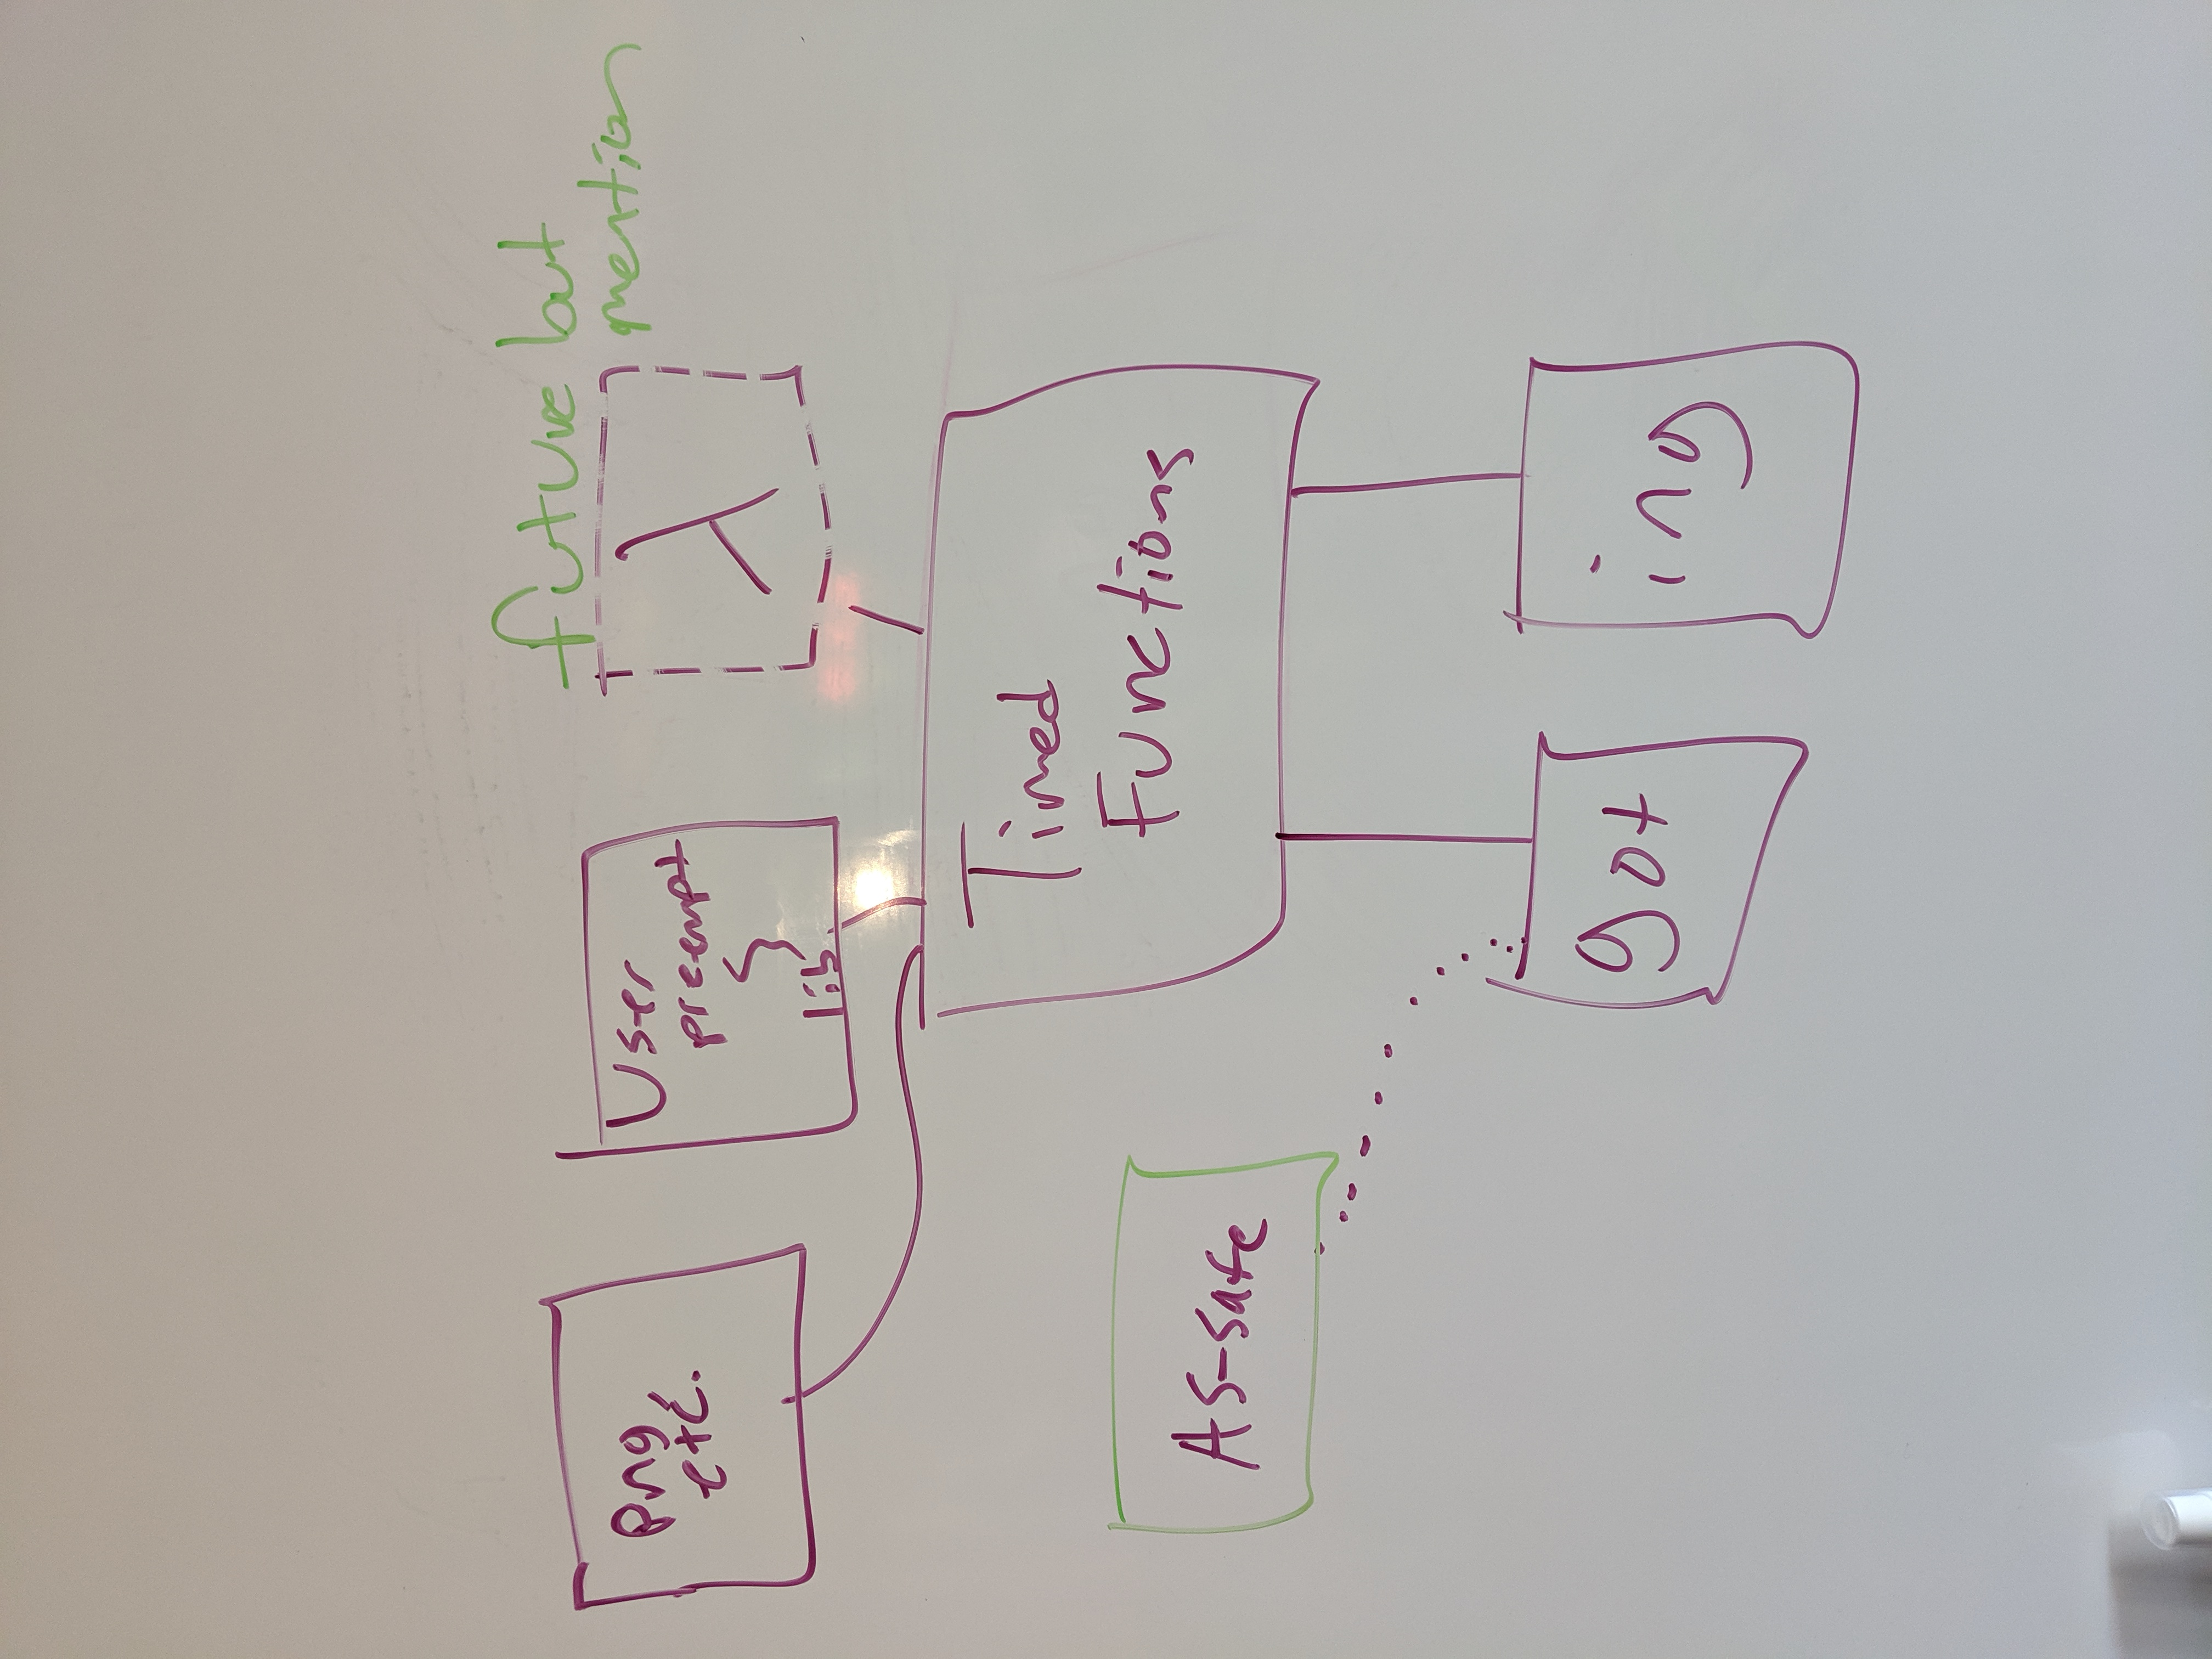
\includegraphics[width=\columnwidth]{figs/architecture}
\end{center}
\caption{Preemptible functions software stack.  \textnormal{Hexagonal boxes show
the required runtime environment.  Rectangular boxes represent components
implementing the preemptible functions abstraction.  Ovals represent components built
on top of these.  A preemptible function's body (e.g., $F$) may be defined directly in
your program, or in some other loaded library.}}
\label{fig:architecture}
\end{figure}

\solb{THESIS: Give a tour of \textit{libtimetravel}?}


\subsection{Automatic handling of shared state}
\label{sec:libinger:reentrancy}

As we found in Section~\ref{sec:intro}, a key design challenge facing
\textit{libinger} is the shared state problem:  Suppose a preemptible function
$F_0$ calls a stateful routine in a third-party library $L$, and
that $F_0$ times out and is preempted by \textit{libinger}.  Later, the
user invokes another timed function $F_0'$, which also calls a stateful
routine in $L$.  This constituting a concurrency violation,
\textit{libinger} must hide state modifications in $L$ by $F_0$
from the execution of $F_0'$ to avoid undefined behavior.

The problem is actually even worse.  Those familiar with POSIX signals may notice
that, upon a function's timeout, its caller interrupts it.  \textit{The rest of the
program} can therefore be viewed as a signal handler, and would normally be expected
to restrict itself to calling async-signal-safe (roughly, nonreentrant)
functions~\cite{signal-safety-manpage}.

One non-solution to this problem is to instead prevent \textit{preemptible functions}
from
calling into third-party code, but doing so would
severely limit their usefulness (Section~\ref{sec:related}).  We opt instead
to automatically and dynamically create copies of $L$ to
isolate state from different timed functions.  Making this work on top of
existing systems software required solving many
design and implementation challenges, which we cover when we introduce
\textit{libgotcha} in Section~\ref{sec:libgotcha}.


\subsection{Safe concurrency}
\label{sec:libinger:concurrency}

Automatically handling shared state arising from nonreentrant library interfaces is
needed because the sharing is transparent to the programmer.  A
different problem arises when a programmer explicitly shares state between a
preemptible function and any other part of the program.  Unlike third-party library
authors, this programmer knows they are using preemptible functions, a
concurrency mechanism.

When using the C interface, the programmer bears complete responsibility for writing
race-free code (e.g., by using atomics and mutexes wherever necessary).
The \textit{libinger} Rust API, however, leverages the
language's first-class concurrency support to prevent such mistakes from compiling:\@
\texttt{launch()}'s signature requires the wrapped function to be \texttt{Send} safe
(only reference state in a thread-safe manner)~\cite{www-rustlang-conc}.

While the Rust compiler rejects all code that shares state unsafely, it is still
possible to introduce
correctness bugs such as deadlock~\cite{www-rustlang-nu}.  One way to do this is to
block on a mutex held by
the preemptible function's caller (recall that invocation is synchronous, so blocking
in a preemptible function does not cause it to yield!).  It is sometimes necessary to
acquire such a mutex, so \textit{libinger} provides a way to do it:  The API has one
last function, \texttt{pause()}, that is a rough analog of yield.  After performing a
try-lock operation, a preemptible function can call this function to immediately
return to its caller as if it had timed out.  The caller can detect this by checking
a flag on the continuation.


\subsection{Execution stacks}

When a preemptible function times out, \textit{libinger} returns a
continuation object.  The caller might pass this object around the program, which
could later call \texttt{resume()} from a different stack frame.  Thus, the
continuation must contain not only the register context, but also the stack
frames belonging to the preemptible function and its callees.  The \texttt{launch()}
function enables this by switching to a new, dedicated stack just before invoking the
user-provided function.

Because of the infeasibility of moving these stacks after a function has started
executing, \textit{libinger} currently heap-allocates large 2-MB stacks so it can
treat them as having fixed size.  To avoid an order of magnitude slowdown from having
such large dynamic allocations on the critical path, \textit{libinger} preallocates a
pool of reusable stacks when it is first used.


\subsection{Timer interrupts}
\label{sec:libinger:signals}

\begin{figure}
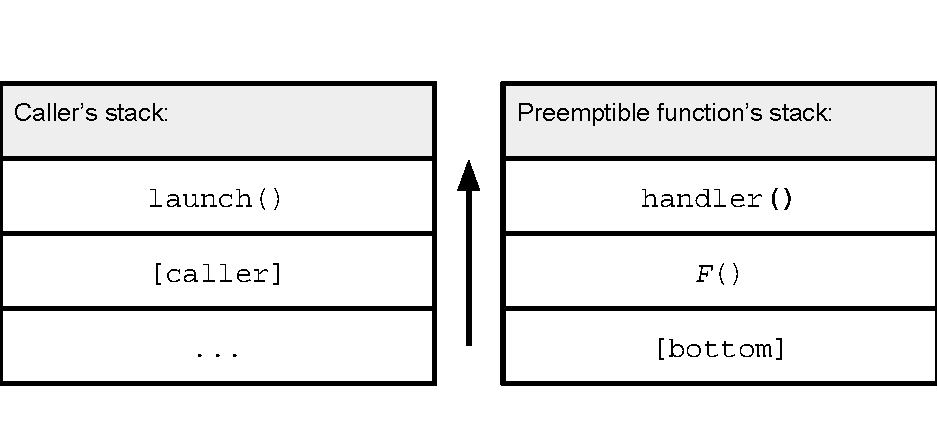
\includegraphics[width=\columnwidth]{figs/twostacks}
\caption{The stacks just before a timeout.  \textnormal{Upon discovering
that the preemptible function has exceeded its time bound, the handler jumps into the
\texttt{launch()} (or \texttt{resume()}) function, which in turn returns to the
original call site, removing its own stack frame in the process.}}
\label{fig:twostacks}
\end{figure}

Whenever \textit{libinger} is executing a user-provided function, we
enable fine-grained timer interrupts to
monitor that function's elapsed running time.  A timer interrupt fires
periodically\footnote{For simplicity, we use a fixed signal frequency for all
preemptible functions, but this is not fundamental to the design.  In the future,
we plan to adjust each function's frequency based on its timeout, and to delay the
first signal until shortly before the time limit (in the case of longer-running
functions).}, causing our signal
handler to be invoked.  If the function exceeds its timeout,
this handler saves a continuation by dumping the machine's registers.  It then
performs an unstructured jump out of the signal handler and back into the
\texttt{launch()} or \texttt{resume()} function, switching stacks as it does so.
Figure~\ref{fig:twostacks} shows the two stacks of execution
that are present while the
signal handler is running.

A subsequent \texttt{resume()} call restores the registers from the stored
continuation, thereby jumping back into the signal handler.  The handler
returns, resuming the preemptible function from the instruction that was executing
when the preemption signal arrived.


\solb{THESIS: Removed discussion of our signal pool trick for notifying specific
POSIX threads.}

\solb{THESIS: Removed discussion of our self-signaling trick for restoring a signal
handler's POSIX context without using \texttt{setcontext()}.}


\subsection{Cancellation}

Should a caller decide not to finish running a timed-out preemptible function, it
must deallocate it.  In Rust this happens implicitly via the \texttt{linger\_t}
type's destructor, whereas users of the C interface are responsible for explicitly
calling the \textit{libinger} \texttt{cancel()} function.

Cancellation cleans up the \textit{libinger} resources allocated by
\texttt{launch()};
however, the current implementation
does not automatically release resources already claimed by the
preemptible function itself.  While the lack of a standard resource deallocation API
makes this inherently hard to do in C, it is possible in languages
such as Rust that support destructors.  For instance, the approach proposed by
Boucher et al.~\cite{boucher:atc2018} could be employed to raise a panic
(exception) on the preemptible function's stack.  This in turn would cause the
language runtime
to unwind each stack frame, invoking local variables' destructors in
the process.

\solb{THESIS: Implement resource cleanup.}
